\subsection*{Propositions}

\begin{remark*}[Source note]
The following propositions are selected from Euclid's Book I in modern theorem
form, following the Heath translation of the \textit{Elements}
\citep[Book I]{euclid-elements-heath}. The selection is curated for the
trigonometric construction: congruence, parallel-angle control, triangle
angle-sum, area comparison, square construction, and the Pythagorean theorem.
\end{remark*}


\begin{theorembox}{Theorem}
\begin{theorem}[Euclid I.1: Constructing an equilateral triangle]
\label{thm:euclid-i-1}
\label{prop:I.1}
Given a finite straight line segment $AB$, there exists an equilateral
triangle $ABC$ constructed on $AB$.
\hyperref[prf:euclid-i-1]{\textit{Go to proof.}}
\end{theorem}
\end{theorembox}
\begin{center}
\begin{tikzpicture}[scale=1.35, line cap=round, line join=round]
  \definecolor{euclidblue}{RGB}{30,110,190}
  \tikzset{
    equaltick/.style={
      postaction={decorate},
      decoration={markings, mark=at position 0.5 with {
        \draw[line width=0.6pt] (0,-2.4pt)--(0,2.4pt);
      }}
    }
  }

  \coordinate (A) at (0,0);
  \coordinate (B) at (2.2,0);
  \pgfmathsetmacro{\R}{2.2}
  \coordinate (C) at (1.1,{sqrt(3)/2*\R});

  \draw[gray!55, thin] (A) circle (\R);
  \draw[gray!55, thin] (B) circle (\R);

  \draw[very thick, equaltick] (A) -- (B);
  \draw[very thick, euclidblue, equaltick] (A) -- (C);
  \draw[very thick, euclidblue, equaltick] (B) -- (C);

  \foreach \p/\pos in {A/below left,B/below right,C/above}{
    \fill (\p) circle (0.025);
    \node[\pos] at (\p) {$\p$};
  }

  \node[gray!70, font=\footnotesize] at ($(A)+(-1.00,-1.10)$) {center $A$};
  \node[gray!70, font=\footnotesize] at ($(B)+(1.00,-1.10)$) {center $B$};
  \node[euclidblue, font=\footnotesize] at ($(A)!0.5!(C)+(-0.24,0.06)$) {$=AB$};
  \node[euclidblue, font=\footnotesize] at ($(B)!0.5!(C)+(0.28,0.06)$) {$=AB$};
\end{tikzpicture}
\end{center}

\begin{remark*}[Proof]
\hyperref[prf:euclid-i-1]{Go to proof.}
\end{remark*}
\begin{remark*}[Standard quantified statement]
This is a classical Euclidean source-text clause. In this chapter it is treated
as a named primitive statement rather than expanded into a modern first-order
formalization.
\end{remark*}
\begin{lra-not-visible}
\begin{dependencies}
\begin{itemize}
  \item \hyperref[def:euclid-point]{Point}
  \item \hyperref[def:euclid-straight-line]{Straight line}
  \item \hyperref[def:euclid-circle]{Circle}
  \item \hyperref[def:euclid-triangle-side-classes]{Equilateral triangle}
  \item \hyperref[ax:euclid-postulate-draw-straight-line]{Euclid Postulate I}
  \item \hyperref[ax:euclid-postulate-describe-circle]{Euclid Postulate III}
  \item \hyperref[ax:euclid-common-notion-things-equal-to-same]{Euclid Common Notion I}
\end{itemize}
\end{dependencies}
\end{lra-not-visible}

\begin{theorembox}{Theorem}
\begin{theorem}[Euclid I.2: Copying a segment from a given point]
\label{thm:euclid-i-2}
\label{prop:I.2}
Given a point $A$ and a finite straight line segment $BC$, there exists a
straight line segment beginning at $A$ and equal to $BC$.
\hyperref[prf:euclid-i-2]{\textit{Go to proof.}}
\end{theorem}
\end{theorembox}
\begin{center}
\begin{tikzpicture}[scale=1.15, line cap=round, line join=round]
  \definecolor{euclidblue}{RGB}{30,110,190}
  \tikzset{
    equaltick/.style={
      postaction={decorate},
      decoration={markings, mark=at position 0.5 with {
        \draw[line width=0.6pt] (0,-2.4pt)--(0,2.4pt);
      }}
    }
  }

  \coordinate (A) at (0,0);
  \coordinate (B) at (2.1,0);
  \coordinate (C) at (3.0,0);
  \coordinate (D) at (1.05,1.65);
  \pgfmathsetmacro{\seg}{0.9}
  \pgfmathsetmacro{\db}{sqrt((2.1-1.05)^2+(0-1.65)^2)}
  \pgfmathsetmacro{\scaleG}{\seg/\db}
  \coordinate (G) at ($(B)+\scaleG*(B)-\scaleG*(D)$);
  \pgfmathsetmacro{\dg}{\db+\seg}
  \coordinate (L) at ($(D)!\dg/\db!(A)$);

  \draw[gray!50, thin] (B) circle (\seg);
  \draw[gray!45, thin] (D) circle (\dg);

  \draw[gray!70, thin] (D) -- ($(D)!1.45!(A)$);
  \draw[gray!70, thin] (D) -- ($(D)!1.45!(B)$);
  \draw[gray!70, thin] (A) -- (B);
  \draw[gray!70, thin] (D) -- (A) -- (B) -- cycle;

  \draw[very thick, equaltick] (B) -- (C);
  \draw[very thick, euclidblue, equaltick] (A) -- (L);
  \draw[very thick, euclidblue] (B) -- (G);
  \draw[very thick, euclidblue] (D) -- (G);
  \draw[very thick, euclidblue] (D) -- (L);

  \foreach \p/\pos in {A/below,B/below,C/below,G/below right,D/above,L/below left}{
    \fill (\p) circle (0.023);
    \node[\pos] at (\p) {$\p$};
  }

  \node[font=\footnotesize] at ($(B)!0.5!(C)+(0,-0.28)$) {$BC$};
  \node[euclidblue, font=\footnotesize] at ($(A)!0.5!(L)+(-0.20,-0.16)$) {$AL=BC$};
  \node[gray!70, font=\footnotesize] at ($(B)+(0.65,-0.70)$) {center $B$};
  \node[gray!70, font=\footnotesize] at ($(D)+(-1.00,1.05)$) {center $D$};
\end{tikzpicture}
\end{center}

\begin{remark*}[Proof]
\hyperref[prf:euclid-i-2]{Go to proof.}
\end{remark*}
\begin{remark*}[Standard quantified statement]
This is a classical Euclidean source-text clause. In this chapter it is treated
as a named primitive statement rather than expanded into a modern first-order
formalization.
\end{remark*}
\begin{lra-not-visible}
\begin{dependencies}
\begin{itemize}
  \item \hyperref[def:euclid-point]{Point}
  \item \hyperref[def:euclid-straight-line]{Straight line}
  \item \hyperref[def:euclid-circle]{Circle}
  \item \hyperref[thm:euclid-i-1]{Euclid I.1}
  \item \hyperref[ax:euclid-postulate-draw-straight-line]{Euclid Postulate I}
  \item \hyperref[ax:euclid-postulate-produce-straight-line]{Euclid Postulate II}
  \item \hyperref[ax:euclid-postulate-describe-circle]{Euclid Postulate III}
  \item \hyperref[ax:euclid-common-notion-things-equal-to-same]{Euclid Common Notion I}
\end{itemize}
\end{dependencies}
\end{lra-not-visible}

\begin{theorembox}{Theorem}
\begin{theorem}[Euclid I.3: Cutting off an equal segment]
\label{thm:euclid-i-3}
\label{prop:I.3}
Given two unequal finite straight line segments, there exists a construction
which cuts off from the greater a straight line segment equal to the less.
\hyperref[prf:euclid-i-3]{\textit{Go to proof.}}
\end{theorem}
\end{theorembox}
\begin{center}
\begin{tikzpicture}[scale=1.2, line cap=round, line join=round]
  \definecolor{euclidblue}{RGB}{30,110,190}
  \tikzset{
    equaltick/.style={
      postaction={decorate},
      decoration={markings, mark=at position 0.5 with {
        \draw[line width=0.6pt] (0,-2.4pt)--(0,2.4pt);
      }}
    }
  }

  \coordinate (A) at (0,0);
  \coordinate (E) at (1.55,0);
  \coordinate (B) at (3.7,0);
  \coordinate (C) at (0,-0.9);
  \coordinate (D) at (1.55,-0.9);
  \pgfmathsetmacro{\r}{1.55}

  \draw[gray!50, thin] (A) circle (\r);
  \draw[very thick] (A) -- (B);
  \draw[very thick, equaltick] (C) -- (D);
  \draw[very thick, euclidblue, equaltick] (A) -- (E);

  \foreach \p/\pos in {A/above left,E/above,B/above right,C/below left,D/below right}{
    \fill (\p) circle (0.023);
    \node[\pos] at (\p) {$\p$};
  }

  \node[font=\footnotesize] at ($(A)!0.5!(B)+(0,0.27)$) {greater segment};
  \node[font=\footnotesize] at ($(C)!0.5!(D)+(0,-0.28)$) {less segment};
  \node[euclidblue, font=\footnotesize] at ($(A)!0.5!(E)+(0,0.34)$) {$AE=CD$};
  \node[gray!70, font=\footnotesize] at ($(A)+(-0.50,-1.50)$) {center $A$};
\end{tikzpicture}
\end{center}

\begin{remark*}[Proof]
\hyperref[prf:euclid-i-3]{Go to proof.}
\end{remark*}
\begin{remark*}[Standard quantified statement]
This is a classical Euclidean source-text clause. In this chapter it is treated
as a named primitive statement rather than expanded into a modern first-order
formalization.
\end{remark*}
\begin{lra-not-visible}
\begin{dependencies}
\begin{itemize}
  \item \hyperref[def:euclid-straight-line]{Straight line}
  \item \hyperref[def:euclid-circle]{Circle}
  \item \hyperref[thm:euclid-i-2]{Euclid I.2}
  \item \hyperref[ax:euclid-postulate-describe-circle]{Euclid Postulate III}
  \item \hyperref[ax:euclid-common-notion-things-equal-to-same]{Euclid Common Notion I}
\end{itemize}
\end{dependencies}
\end{lra-not-visible}

\begin{theorembox}{Theorem}
\begin{theorem}[Euclid I.4: Side-angle-side congruence]
\label{thm:euclid-i-4}
If two triangles have two sides equal to two sides respectively, and have the
angles contained by the equal straight lines equal, then they also have the
base equal to the base, the triangle equal to the triangle, and the remaining
angles equal to the remaining angles respectively.
\hyperref[prf:euclid-i-4]{\textit{Go to proof.}}
\end{theorem}
\end{theorembox}
\begin{center}
\begin{tikzpicture}[scale=0.95, line cap=round, line join=round]
  \definecolor{euclidblue}{RGB}{30,110,190}
  \tikzset{
    onetick/.style={postaction={decorate},decoration={markings,mark=at position 0.5 with {\draw (0,-2pt)--(0,2pt);}}},
    twotick/.style={postaction={decorate},decoration={markings,mark=at position 0.45 with {\draw (0,-2pt)--(0,2pt);},mark=at position 0.55 with {\draw (0,-2pt)--(0,2pt);}}}
  }
  \coordinate (A) at (0,0);
  \coordinate (B) at (2.6,0);
  \coordinate (C) at (1.0,1.8);
  \coordinate (D) at (4.3,0);
  \coordinate (E) at (6.9,0);
  \coordinate (F) at (5.3,1.8);
  \draw[very thick, onetick] (A)--(B);
  \draw[very thick, twotick] (A)--(C);
  \draw[very thick, euclidblue] (B)--(C);
  \draw[very thick, onetick] (D)--(E);
  \draw[very thick, twotick] (D)--(F);
  \draw[very thick, euclidblue] (E)--(F);
  \draw (0.38,0) arc[start angle=0,end angle=61,radius=0.38];
  \draw ($(D)+(0.38,0)$) arc[start angle=0,end angle=61,radius=0.38];
  \foreach \p/\pos in {A/below left,B/below,C/above,D/below left,E/below,F/above}{
    \fill (\p) circle (0.026);
    \node[\pos] at (\p) {$\p$};
  }
  \node[font=\footnotesize] at (1.35,-0.45) {$AB=DE$};
  \node[font=\footnotesize] at (5.62,-0.45) {$AC=DF$};
  \node[euclidblue, font=\footnotesize] at (3.45,1.15) {included angles equal};
\end{tikzpicture}
\end{center}

\begin{remark*}[Proof]
\hyperref[prf:euclid-i-4]{Go to proof.}
\end{remark*}
\begin{remark*}[Standard quantified statement]
This is a classical Euclidean source-text clause. In this chapter it is treated
as a named primitive statement rather than expanded into a modern first-order
formalization.
\end{remark*}
\begin{lra-not-visible}
\begin{dependencies}
\begin{itemize}
  \item \hyperref[def:euclid-triangle-side-classes]{Triangle side classes}
  \item \hyperref[def:euclid-rectilinear-angle]{Rectilinear angle}
  \item \hyperref[ax:euclid-common-notion-coinciding-things-equal]{Euclid Common Notion IV}
\end{itemize}
\end{dependencies}
\end{lra-not-visible}

\begin{theorembox}{Theorem}
\begin{theorem}[Euclid I.31: Drawing a parallel through a point]
\label{thm:euclid-i-31}
Through a given point, to draw a straight line parallel to a given straight
line.
\hyperref[prf:euclid-i-31]{\textit{Go to proof.}}
\end{theorem}
\end{theorembox}
\begin{center}
\begin{tikzpicture}[scale=1.05, line cap=round, line join=round]
  \definecolor{euclidblue}{RGB}{30,110,190}
  \coordinate (A) at (-2.8,0);
  \coordinate (B) at (2.8,0);
  \coordinate (P) at (-0.7,1.65);
  \coordinate (Q) at (2.6,1.65);
  \draw[very thick] (A)--(B);
  \draw[very thick, euclidblue] ($(P)!-0.55!(Q)$)--($(P)!1.25!(Q)$);
  \draw[gray!65, dashed] (P)--(0.2,0);
  \draw[gray!65, dashed] (P)--(1.1,0);
  \foreach \p/\pos in {A/below,B/below,P/above,Q/above}{
    \fill (\p) circle (0.026);
    \node[\pos] at (\p) {$\p$};
  }
  \node[font=\footnotesize] at (0,-0.35) {given straight line};
  \node[euclidblue, font=\footnotesize] at (1.2,1.98) {parallel through $P$};
  \node[gray!70, font=\footnotesize] at (0.30,0.78) {equal alternate angles};
\end{tikzpicture}
\end{center}

\begin{remark*}[Proof]
\hyperref[prf:euclid-i-31]{Go to proof.}
\end{remark*}
\begin{remark*}[Standard quantified statement]
This is a classical Euclidean source-text clause. In this chapter it is treated
as a named primitive statement rather than expanded into a modern first-order
formalization.
\end{remark*}
\begin{lra-not-visible}
\begin{dependencies}
\begin{itemize}
  \item \hyperref[def:euclid-parallel-straight-lines]{Parallel straight lines}
  \item \hyperref[ax:euclid-postulate-draw-straight-line]{Euclid Postulate I}
  \item \hyperref[ax:euclid-postulate-parallel]{Euclid Postulate V}
\end{itemize}
\end{dependencies}
\end{lra-not-visible}

\begin{theorembox}{Theorem}
\begin{theorem}[Euclid I.32: Triangle angle sum]
\label{thm:euclid-i-32}
In any triangle, if one of the sides is produced, then the exterior angle is
equal to the two interior and opposite angles, and the three interior angles of
the triangle are equal to two right angles.
\hyperref[prf:euclid-i-32]{\textit{Go to proof.}}
\end{theorem}
\end{theorembox}
\begin{center}
\begin{tikzpicture}[scale=1.1, line cap=round, line join=round]
  \definecolor{euclidblue}{RGB}{30,110,190}
  \coordinate (A) at (0,0);
  \coordinate (B) at (3.2,0);
  \coordinate (C) at (1.1,1.85);
  \coordinate (L) at ($(C)+(-1.5,0)$);
  \coordinate (R) at ($(C)+(2.4,0)$);
  \draw[very thick] (A)--(B)--(C)--cycle;
  \draw[very thick, euclidblue] (L)--(R);
  \draw ($(A)+(0.34,0)$) arc[start angle=0,end angle=59,radius=0.34];
  \draw ($(B)+(-0.34,0)$) arc[start angle=180,end angle=139,radius=0.34];
  \draw ($(C)+(-118:0.34)$) arc[start angle=-118,end angle=-41,radius=0.34];
  \foreach \p/\pos in {A/below left,B/below right,C/above,L/left,R/right}{
    \fill (\p) circle (0.024);
    \node[\pos] at (\p) {$\p$};
  }
  \node[euclidblue, font=\footnotesize] at ($(C)+(1.05,0.28)$) {parallel to $AB$};
  \node[font=\footnotesize] at (1.55,-0.34) {$\angle A+\angle B+\angle C=2$ right angles};
\end{tikzpicture}
\end{center}

\begin{remark*}[Proof]
\hyperref[prf:euclid-i-32]{Go to proof.}
\end{remark*}
\begin{remark*}[Standard quantified statement]
This is a classical Euclidean source-text clause. In this chapter it is treated
as a named primitive statement rather than expanded into a modern first-order
formalization.
\end{remark*}
\begin{lra-not-visible}
\begin{dependencies}
\begin{itemize}
  \item \hyperref[def:euclid-triangle-angle-classes]{Triangle angle classes}
  \item \hyperref[thm:euclid-i-31]{Euclid I.31}
  \item \hyperref[ax:euclid-postulate-parallel]{Euclid Postulate V}
\end{itemize}
\end{dependencies}
\end{lra-not-visible}

\begin{theorembox}{Theorem}
\begin{theorem}[Euclid I.41: Triangle and parallelogram on the same base]
\label{thm:euclid-i-41}
If a parallelogram has the same base with a triangle and is in the same
parallels, then the parallelogram is double the triangle.
\hyperref[prf:euclid-i-41]{\textit{Go to proof.}}
\end{theorem}
\end{theorembox}
\begin{center}
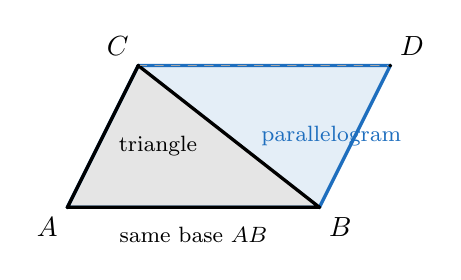
\begin{tikzpicture}[scale=1.0, line cap=round, line join=round]
  \definecolor{euclidblue}{RGB}{30,110,190}
  \coordinate (A) at (0,0);
  \coordinate (B) at (3.2,0);
  \coordinate (C) at (0.9,1.8);
  \coordinate (D) at (4.1,1.8);
  \fill[euclidblue!12] (A)--(B)--(D)--(C)--cycle;
  \fill[gray!20] (A)--(B)--(C)--cycle;
  \draw[very thick, euclidblue] (A)--(B)--(D)--(C)--cycle;
  \draw[very thick] (A)--(B)--(C)--cycle;
  \draw[gray!70, dashed] (C)--(D);
  \foreach \p/\pos in {A/below left,B/below right,C/above left,D/above right}{
    \fill (\p) circle (0.025);
    \node[\pos] at (\p) {$\p$};
  }
  \node[font=\footnotesize] at (1.6,-0.35) {same base $AB$};
  \node[euclidblue, font=\footnotesize] at (3.35,0.9) {parallelogram};
  \node[font=\footnotesize] at (1.15,0.78) {triangle};
\end{tikzpicture}
\end{center}

\begin{remark*}[Proof]
\hyperref[prf:euclid-i-41]{Go to proof.}
\end{remark*}
\begin{remark*}[Standard quantified statement]
This is a classical Euclidean source-text clause. In this chapter it is treated
as a named primitive statement rather than expanded into a modern first-order
formalization.
\end{remark*}
\begin{lra-not-visible}
\begin{dependencies}
\begin{itemize}
  \item \hyperref[def:euclid-parallel-straight-lines]{Parallel straight lines}
  \item \hyperref[def:euclid-quadrilateral-classes]{Quadrilateral classes}
  \item \hyperref[ax:euclid-common-notion-coinciding-things-equal]{Euclid Common Notion IV}
\end{itemize}
\end{dependencies}
\end{lra-not-visible}

\begin{theorembox}{Theorem}
\begin{theorem}[Euclid I.46: Constructing a square on a segment]
\label{thm:euclid-i-46}
On a given straight line, to describe a square.
\hyperref[prf:euclid-i-46]{\textit{Go to proof.}}
\end{theorem}
\end{theorembox}
\begin{center}
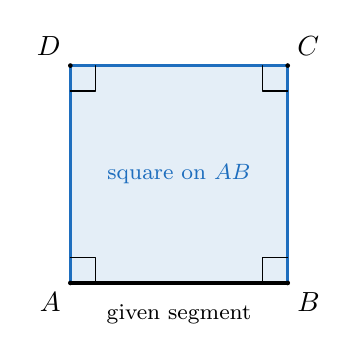
\begin{tikzpicture}[scale=1.15, line cap=round, line join=round]
  \definecolor{euclidblue}{RGB}{30,110,190}
  \coordinate (A) at (0,0);
  \coordinate (B) at (2.4,0);
  \coordinate (C) at (2.4,2.4);
  \coordinate (D) at (0,2.4);
  \fill[euclidblue!12] (A)--(B)--(C)--(D)--cycle;
  \draw[very thick, euclidblue] (A)--(B)--(C)--(D)--cycle;
  \draw[very thick] (A)--(B);
  \draw (0.28,0)--(0.28,0.28)--(0,0.28);
  \draw (2.12,0)--(2.12,0.28)--(2.4,0.28);
  \draw (2.12,2.4)--(2.12,2.12)--(2.4,2.12);
  \draw (0.28,2.4)--(0.28,2.12)--(0,2.12);
  \foreach \p/\pos in {A/below left,B/below right,C/above right,D/above left}{
    \fill (\p) circle (0.026);
    \node[\pos] at (\p) {$\p$};
  }
  \node[font=\footnotesize] at (1.2,-0.35) {given segment};
  \node[euclidblue, font=\footnotesize] at (1.2,1.2) {square on $AB$};
\end{tikzpicture}
\end{center}

\begin{remark*}[Proof]
\hyperref[prf:euclid-i-46]{Go to proof.}
\end{remark*}
\begin{remark*}[Standard quantified statement]
This is a classical Euclidean source-text clause. In this chapter it is treated
as a named primitive statement rather than expanded into a modern first-order
formalization.
\end{remark*}
\begin{lra-not-visible}
\begin{dependencies}
\begin{itemize}
  \item \hyperref[def:euclid-quadrilateral-classes]{Square}
  \item \hyperref[thm:euclid-i-31]{Euclid I.31}
  \item \hyperref[ax:euclid-postulate-draw-straight-line]{Euclid Postulate I}
  \item \hyperref[ax:euclid-postulate-right-angles-equal]{Euclid Postulate IV}
\end{itemize}
\end{dependencies}
\end{lra-not-visible}

\begin{theorembox}{Theorem}
\begin{theorem}[Euclid I.47: Pythagorean theorem]
\label{thm:euclid-i-47}
\label{prop:I.47}
In right-angled triangles, the square on the side subtending the right angle is
equal to the squares on the sides containing the right angle.
\hyperref[prf:euclid-i-47]{\textit{Go to proof.}}
\end{theorem}
\end{theorembox}
\begin{center}
\begin{tikzpicture}[scale=0.78, line cap=round, line join=round]
  \definecolor{euclidblue}{RGB}{30,110,190}
  \definecolor{euclidred}{RGB}{180,70,55}
  \definecolor{euclidgreen}{RGB}{65,135,85}

  \coordinate (A) at (0,0);
  \coordinate (B) at (4,0);
  \coordinate (C) at (0,3);
  \coordinate (AB1) at (0,-4);
  \coordinate (AB2) at (4,-4);
  \coordinate (AC1) at (-3,0);
  \coordinate (AC2) at (-3,3);
  \coordinate (BC1) at ($(B)+(3,4)$);
  \coordinate (BC2) at ($(C)+(3,4)$);

  \fill[euclidblue!13] (A) -- (B) -- (AB2) -- (AB1) -- cycle;
  \fill[euclidgreen!13] (A) -- (AC1) -- (AC2) -- (C) -- cycle;
  \fill[euclidred!13] (B) -- (BC1) -- (BC2) -- (C) -- cycle;

  \draw[very thick] (A) -- (B) -- (C) -- cycle;
  \draw[thick, euclidblue] (A) -- (B) -- (AB2) -- (AB1) -- cycle;
  \draw[thick, euclidgreen] (A) -- (AC1) -- (AC2) -- (C) -- cycle;
  \draw[thick, euclidred] (B) -- (BC1) -- (BC2) -- (C) -- cycle;

  \draw[thin] ($(A)+(0.34,0)$) -- ($(A)+(0.34,0.34)$) -- ($(A)+(0,0.34)$);
  \draw[dashed, gray!60] (A) -- ($(A)+(3.0,-4.0)$);
  \draw[dashed, gray!60] (C) -- ($(C)+(3.0,-4.0)$);

  \foreach \p/\pos in {A/below left,B/below right,C/above left}{
    \fill (\p) circle (0.035);
    \node[\pos] at (\p) {$\p$};
  }

  \node[euclidblue] at (2,-2.2) {square on $AB$};
  \node[euclidgreen, rotate=90] at (-1.75,1.5) {square on $AC$};
  \node[euclidred, rotate=53] at ($(B)!0.5!(BC2)+(1.1,1.0)$) {square on $BC$};
  \node[font=\footnotesize] at (0.65,0.42) {right angle};
\end{tikzpicture}
\end{center}

\begin{remark*}[Proof]
\hyperref[prf:euclid-i-47]{Go to proof.}
\end{remark*}
\begin{remark*}[Placement]
This proposition is pulled forward as the Book I capstone needed by the
trigonometric definitions. Its professional proof depends on later Book I
propositions that are not yet developed in this chapter; the proof file records
those pending Euclidean nodes explicitly.
\end{remark*}
\begin{lra-not-visible}
\begin{dependencies}
\begin{itemize}
  \item \hyperref[def:euclid-right-angle-and-perpendicular]{Right angle and perpendicular}
  \item \hyperref[def:euclid-triangle-angle-classes]{Right-angled triangle}
  \item \hyperref[def:euclid-quadrilateral-classes]{Square}
  \item \hyperref[ax:euclid-postulate-draw-straight-line]{Euclid Postulate I}
  \item \hyperref[ax:euclid-common-notion-add-equals]{Euclid Common Notion II}
  \item \hyperref[ax:euclid-common-notion-subtract-equals]{Euclid Common Notion III}
  \item \hyperref[thm:euclid-i-4]{Euclid I.4}
  \item \hyperref[thm:euclid-i-41]{Euclid I.41}
  \item \hyperref[thm:euclid-i-46]{Euclid I.46}
\end{itemize}
\end{dependencies}
\end{lra-not-visible}
